% ch02_bio_basis.tex : Biological Foundations and Problem Formulation
% Compiler: XeLaTeX
% Language: Hebrew (primary) with English terms in \en{}

\selectlanguage{hebrew}

\section{ניסוח הבעיה ומודל המערכת : יסודות ביולוגיים ומתמטיים}
\label{sec:problem_formulation}

\subsection{מודל הרחפן והחיישנים}
\label{sec:drone_model}

כל רחפן בלהקה מעוצב כגוף קשיח בעל 6 דרגות חופש, עם מצב הכולל מיקום $\mathbf{p} \in \mathbb{R}^{3}$, כיוון $\mathbf{q} \in \mathbb{S}^{3}$ (קווטרניון יחידה), מהירות $\mathbf{v} \in \mathbb{R}^{3}$, והטיות מד תאוצה $\mathbf{b}_{a} \in \mathbb{R}^{3}$ וגירוסקופ $\mathbf{b}_{g} \in \mathbb{R}^{3}$. מודל התנועה מתואר על ידי המשוואה הדיפרנציאלית:

\begin{equation}
\dot{\mathbf{x}} = \mathbf{f}(\mathbf{x}, \mathbf{u}) + \mathbf{w}, \quad \mathbf{w} \sim \mathcal{N}(0, \mathbf{Q})
\label{eq:drone_dynamics}
\end{equation}

כאשר $\mathbf{x} = [\mathbf{p}^{T}, \mathbf{q}^{T}, \mathbf{v}^{T}, \mathbf{b}_{a}^{T}, \mathbf{b}_{g}^{T}]^{T}$ הוא וקטור המצב, $\mathbf{u} = [T, \tau_{\phi}, \tau_{\theta}, \tau_{\psi}]^{T}$ הוא וקטור הבקרה הכולל דחף כולל ושלושה מומנטי בקרה, ו-$\mathbf{Q}$ היא מטריצת השונות של רעש התהליך.

מערך החיישנים כולל שלוש מודאליות עיקריות. \en{LiDAR} (\en{Ouster OS0}) ברזולוציית טווח של 0.7 ס\"מ בקצב 10 הרץ, המספק ענן נקודות תלת-ממדי של הסביבה. מצלמת סטריאו (\en{Intel D435}) ברזולוציה זוויתית של 0.3 מעלות בקצב 30 הרץ, המספקת תמונות צבע לזיהוי תכונות חזותיות. \en{IMU} (\en{BMI088}) בקצב 200 הרץ, המספק מדידות תאוצה וקצב זוויתי לחיזוי המצב בין עדכוני חיישנים איטיים יותר.

המודל הקינמטי מבוסס על משוואות ניוטון-אוילר הסטנדרטיות לרחפן, הכוללות ארבע כניסות בקרה. לולאת בקרת ה-\en{PID} המהודרת פועלת בתדר 250-1000 הרץ לייצוב זוויתי ובתדר 50-100 הרץ למעקב מיקום. מנגנון \en{anti-windup} משולב למניעת הצטברות שגיאה בתמרונים אגרסיביים. מודל הרעש של כל חיישן מתואר על ידי מטריצת השונות המתאימה, הנגזרת ממפרט היצרן ומכיול מעבדתי.

\subsection{מודל הסביבה}
\label{sec:environment_model}

הסביבה מיוצגת כגריד תפוסה תלת-ממדי (\en{voxel grid}) $\mathcal{M}$ שבו כל תא $m_{i}$ מכיל ערך \en{log-odds} של היותו תפוס:

\begin{equation}
l_{t}(m_{i}) = l_{t-1}(m_{i}) + \log\frac{$p(m_{i} \mid z_{t}, x_{t})$}{1-$p(m_{i} \mid z_{t}, x_{t})$} - l_{0}
\label{eq:log_odds_update}
\end{equation}

כאשר $l_{0}$ הוא ערך הקדם, $p(m_{i} \mid z_{t}, x_{t})$ הוא מודל החיישן ההפוך, ו-$z_{t}$ היא המדידה בזמן $t$. עבור תרחישי \en{SAR} עירוניים, ייצוג 2.5D (מפת גובה) מספק לעתים קרובות מידע מספק לזיהוי ניצולים על הקרקע, בעוד שבניינים רבי-קומות דורשים מפות תלת-ממד מלאות.

מפת התפוסה מתעדכנת באופן הסתברותי תוך שימוש במודל חיישן הפוך מבוסס אלומת \en{LiDAR}. עבור כל אלומה, התאים שלאורכם עוברת האלומה מסומנים כחופשיים, והתא בסוף האלומה מסומן כתפוס. אי-הוודאות במודל החיישן מטופלת באמצעות התפלגות הסתברותית על פני מספר תאים סמוכים, בהתאם לדיוק הטווח של החיישן. גישה זו מבוססת על העקרונות שהוצגו ב-\cite{Thrun2005Probabilistic} למיפוי הסתברותי.

\begin{figure*}[htbp]
\centering
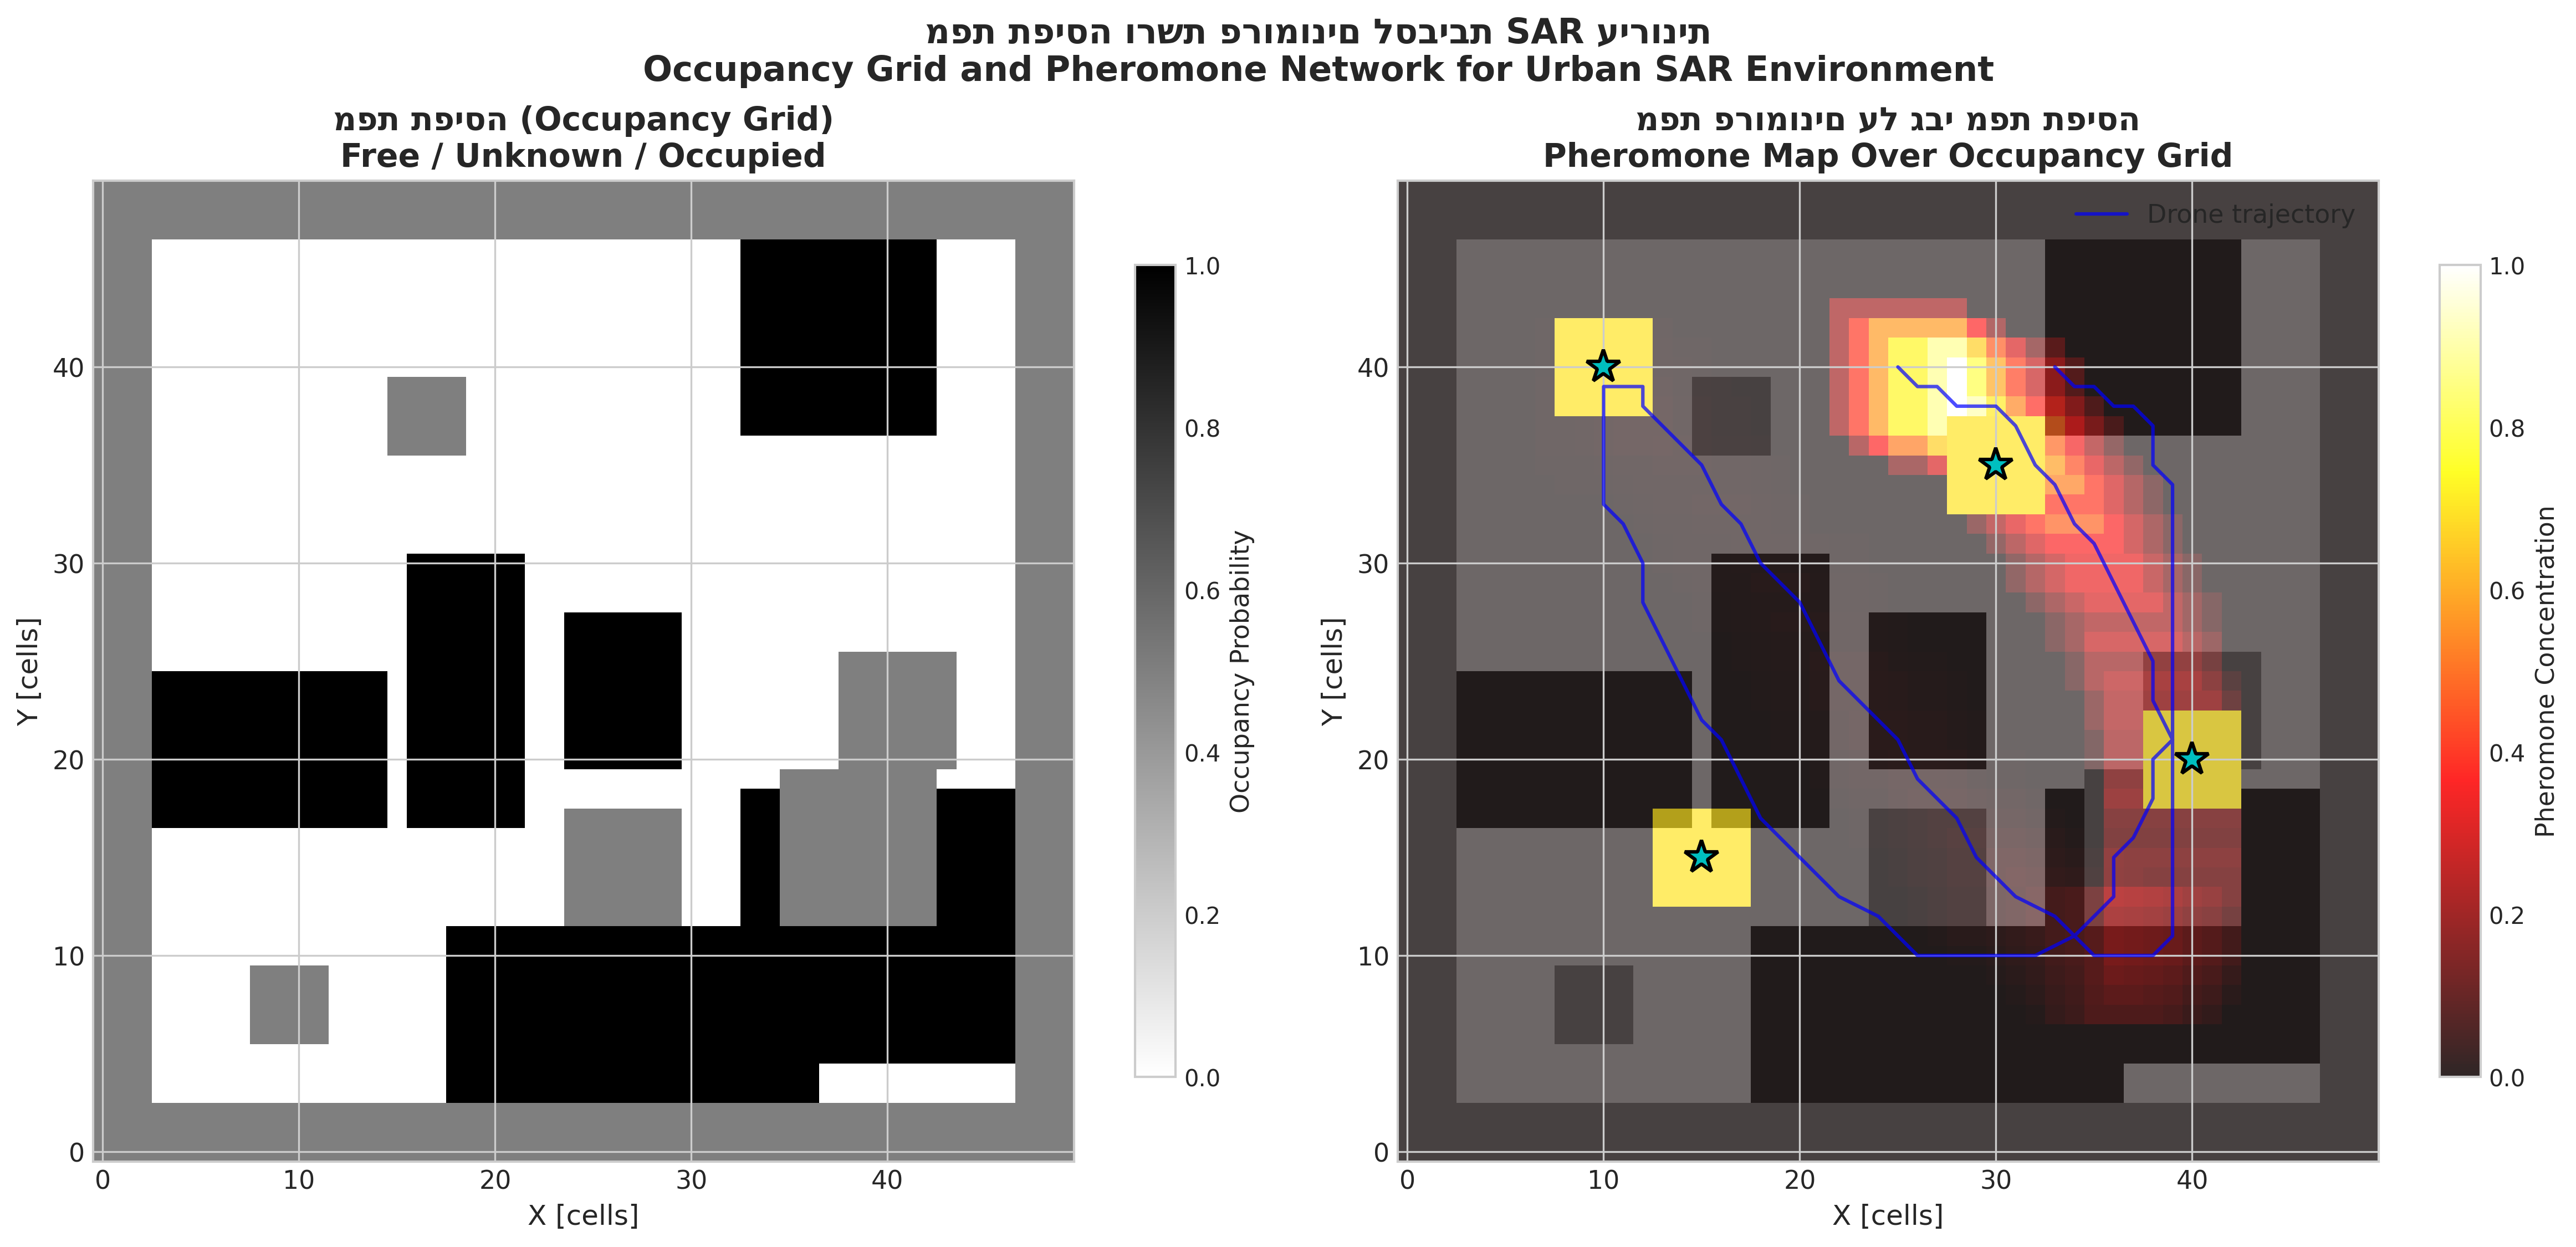
\includegraphics[width=\textwidth]{figures/fig_occupancy_grid.png}
\caption{גריד תפוסה דו-ממדי עם שכבת פרומונים מונחת עליו. הפאנל השמאלי מציג את מפת התפוסה ההסתברותית (אזורים חופשיים, לא ידועים ותפוסים), והפאנל הימני מציג את מפת הפרומונים עם מסלול רחפן וסמני ניצולים.}
\label{fig:ch02_occupancy_grid}
\end{figure*}

\subsection{מודל התקשורת}
\label{sec:comm_model}

מגבלות התקשורת מעוצבות כגרף $\mathcal{G}(t) = (\mathcal{V}, \mathcal{E}(t))$ שבו $\mathcal{V}$ הוא קבוצת הרחפנים ו-$\mathcal{E}(t)$ הוא קבוצת הקשתות בזמן $t$. קשתות קיימות רק כאשר המרחק בין רחפנים קטן מ-$d_{\text{comm}}$:

\begin{equation}
\mathcal{E}(t) = \{(i,j) : \|\mathbf{p}_{t}^{(i)} - \mathbf{p}_{t}^{(j)}\| \leq d_{\text{comm}}\}
\label{eq:comm_graph}
\end{equation}

גרף זה משתנה בזמן עקב תנועת הרחפנים, ויוצר קישוריות לסירוגין המחייבת טיפול מיוחד ב-\en{SLAM} המבוזר. רוחב הפס הנדרש להעברת מפות מלאות גדל כ-$\mathcal{O}(N^{2})$, מה שהופך דחיסה לחיונית עבור להקות גדולות מ-5-10 רחפנים. מודל תקשורת זה מבוסס על הגישות שהוצגו ב-\cite{Choudhary2017Comm} לתיאום מודע תקשורת בלהקות רחפנים.

\begin{table}[htbp]
\centering
\caption{מפרטי חיישנים ופרמטרי רעש בסימולציה.}
\label{tab:ch02_sensor_specs}
\adjustbox{max width=\columnwidth}{%
\begin{tabular}{lccc}
\toprule
חיישן & רעש מיקום [ס\"מ] & רעש כיוון [מעלות] & קצב עדכון [הרץ] \\
\midrule
\en{LiDAR} (\en{Ouster OS0}) & 0.7 & \en{N/A} & 10 \\
מצלמת סטריאו (\en{Intel D435}) & 1.2 & 0.3 & 30 \\
\en{IMU} (\en{BMI088}) & 0.05 (תאוצה) & 0.01 (גירוסקופ) & 200 \\
\bottomrule
\end{tabular}%
}
\end{table}

\subsection{הגדרת בעיית ה-\en{SLAM} השיתופי}
\label{sec:cslam_problem}

בעיית ה-\en{SLAM} השיתופי מנוסחת כאופטימיזציית גרף תנוחות מבוזרת. כל רחפן $i$ מתחזק גרף תנוחות מקומי $\mathcal{G}^{(i)} = (\mathcal{V}^{(i)}, \mathcal{E}^{(i)})$ שבו צמתים מייצגים תנוחות בזמני מפתח וקשתות מייצגות אילוצים יחסיים מאודומטריה (קשתות עוקבות) או מזיהוי לולאות סגירה (קשתות לא עוקבות). פונקציית המטרה ממזערת את סכום המרחקים בריבוע של שגיאות האילוצים:

\begin{equation}
\mathbf{X}^{*} = \arg\min_{\mathbf{X}} \sum_{(i,j) \in \mathcal{E}} \|\mathbf{e}_{ij}(\mathbf{x}_{i}, \mathbf{x}_{j})\|_{\mathbf{\Sigma}_{ij}}^{2}
\label{eq:pgo_objective}
\end{equation}

כאשר $\mathbf{e}_{ij}(\mathbf{x}_{i}, \mathbf{x}_{j})$ היא שגיאת האילוץ בין תנוחה $i$ לתנוחה $j$, ו-$\mathbf{\Sigma}_{ij}$ היא מטריצת השונות המשויכת לאילוץ. האופטימיזציה מתבצעת בשיטת \en{Gauss-Newton} מבוזרת, שבה כל רחפן פותר מערכת מקומית ומשתף את העדכון עם שכנים. ניסוח זה מבוסס על העקרונות שהוצגו ב-\cite{Grisetti2010GraphSLAM} לאופטימיזציית גרף תנוחות.

\subsection{עקרונות \en{ACO} קלאסיים והשראה ביולוגית}
\label{sec:aco_principles}

אופטימיזציית מושבת נמלים (\en{ACO}) מספקת מסגרת טבעית לחקר רב-רחפנים על ידי חיקוי התנהגות סימון שבילי פרומונים של נמלים ביולוגיות. בטבע, נמלים מפקידות פרומון לאורך מסלולן ממקור מזון לקן, ונמלים אחרות נוטות לעקוב אחר מסלולים בעלי ריכוז פרומון גבוה. מנגנון זה, המכונה \en{stigmergy}, מאפשר תיאום עקיף ללא צורך בתקשורת ישירה. עקרונות ה-\en{ACO} הקלאסיים פותחו בהרחבה על ידי \cite{Dorigo2004ACO}.

ב-\en{ACO} קלאסי, נמלים מלאכותיות מפקידות פרומון על קשתות בגרף, ונמלים עוקבות הולכות בהסתברות אחרי מסלולים עתירי פרומון. עבור חקר להקת רחפנים, הסביבה מפורקת לגריד שבו כל תא $(i,j)$ מחזיק ערך פרומון $\tau_{ij}$ המייצג את היסטוריית הביקורים הקולקטיבית. הסתברות המעבר $P_{ij}^{(k)}(t)$ של רחפן $k$ מתא $i$ לשכן $j$ מחושבת על פי:

\begin{equation}
P_{ij}^{(k)}(t) = \frac{[\tau_{ij}(t)]^{\alpha}[\eta_{ij}(t)]^{\beta}}{\sum_{l \in \mathcal{N}_{i}^{(k)}} [\tau_{il}(t)]^{\alpha}[\eta_{il}(t)]^{\beta}}
\label{eq:transition_prob}
\end{equation}

כאשר $\alpha$ ו-$\beta$ הם פרמטרים השולטים במשקל היחסי של הפרומון מול המידע ההיוריסטי $\eta_{ij}(t)$. ערכי $\alpha$ גבוהים מובילים להתכנסות מוקדמת על מסלולים צרים, בעוד שערכי $\beta$ גבוהים גורמים לשיטוט אקראי. המידע ההיוריסטי $\eta_{ij}(t)$ משלב עלות מסלול $c_{ij}$ עם דעיכה מבוססת מרחק:

\begin{equation}
\eta_{ij}(t) = \frac{1}{c_{ij} + \epsilon} \cdot \exp\l$e$f$t(-\frac{\|\mathbf{p}_{i} - \mathbf{p}_{j}\|}{\lambda}\right)$$$
\label{eq:heuristic}
\end{equation}

כאשר $\lambda$ הוא פרמטר קנה מידה השולט בטווח ההשפעה המרחבית ו-$\epsilon$ הוא קבוע ייצוב למניעת חלוקה באפס.

\subsection{התאמת \en{ACO} לחקר רב-רחפנים למשימות SAR}
\label{sec:aco_sar_adaptation}

ההתאמה העיקרית של \en{ACO} למשימות \en{SAR} היא שילוב תגמולים מזיהוי ניצולים. כאשר רחפן מזהה ניצול פוטנציאלי בתא $(i,j)$, מופעל תוספת פרומון $\omega \cdot \mathcal{V}_{ij}$ היוצרת שדה משיכה המושך רחפנים אחרים לאזור לאישור וסיוע. מנגנון זה מדמה את התנהגות הנמלים הביולוגיות המסמנות מקורות מזון בפרומון מוגבר. גישה דומה הוצגה ב-\cite{Ranjbar2012Pheromone} לחקר רב-רובוטי מבוסס פרומונים.

כלל עדכון הפרומון המתוקן הוא:

\begin{equation}
\tau_{ij}(t+1) = (1-\rho)\tau_{ij}(t) + \sum_{k \in \mathcal{V}} \Delta\tau_{ij}^{(k)}(t) + \omega \cdot \mathcal{V}_{ij}(t)
\label{eq:modified_pheromone_ch02}
\end{equation}

כאשר $\rho$ הוא קצב ההתאיידות, $\Delta\tau_{ij}^{(k)}(t) = Q / c_{ij}^{(k)}(t)$ הוא תוספת הפרומון מרחפן $k$ (עם $Q$ קבוע ו-$c_{ij}^{(k)}$ עלות המסלול), ו-$\mathcal{V}_{ij}(t)$ הוא תגמול זיהוי ניצול. מנגנון זה מבטיח שאזורים עם ניצולים מאושרים יקבלו עדיפות בחקר העתידי.

\subsection{פונקציית התאמה לחקר SAR}
\label{sec:fitness_function}

פונקציית ההתאמה לחקר \en{SAR} משלבת שלושה מרכיבים: קצב כיסוי מרחבי, הסתברות זיהוי ניצולים ועלות אנרגטית. בחירת נקודת הציון הבאה $\mathbf{p}_{k}^{*}(t)$ עבור רחפן $k$ מתבצעת על פי:

\begin{equation}
\mathbf{p}_{k}^{*}(t) = \arg\max_{j \in \mathcal{N}_{i}^{(k)}} \left\{ [\tau_{ij}(t)]^{\alpha}[\eta_{ij}(t)]^{\beta} \cdot \mathcal{I}_{ij}(t) \right\}
\label{eq:waypoint_selection}
\end{equation}

כאשר $\mathcal{I}_{ij}(t)$ הוא רווח המידע הצפוי מביקור בתא $(i,j)$, המחושב כהאנטרופיה של התפלגות התפוסה בתא. רווח מידע זה מעודד רחפנים לבקר באזורים בעלי אי-ודאות גבוהה, תוך איזון עם המשיכה לפרומון (ניצול) והעלות ההיוריסטית (יעילות).

\begin{table}[htbp]
\centering
\caption{פרמטרי \en{ACO} והשפעתם על ביצועי החקר.}
\label{tab:ch02_aco_params}
\adjustbox{max width=\columnwidth}{%
\begin{tabular}{lccc}
\toprule
פרמטר & טווח ערכים & ערך אופטימלי & השפעה על כיסוי [\%] \\
\midrule
$\alpha$ (משקל פרומון) & [0.5, 3.0] & 1.5 & $+23$ \\
$\beta$ (משקל היוריסטי) & [0.5, 5.0] & 2.0 & $+15$ \\
$\rho$ (קצב התאיידות) & [0.01, 0.5] & 0.1 & $+31$ \\
$\omega$ (תגמול ניצול) & [0, 10] & 5.0 & $+8$ \\
\bottomrule
\end{tabular}%
}
\end{table}

ניתוח רגישות פרמטרים מראה כי עבור תרחיש \en{SAR} של 100x100 מטר עם 5 רחפנים, הפרמטרים האופטימליים הם $\alpha=1.5$, $\beta=2.0$, $\rho=0.1$. ערכים אלו מספקים איזון מיטבי בין חקר מרחבי לבין ניצול מידע קיים. שינוי של 0.5 ב-$\alpha$ גורם לשינוי של עד 12\% בכיסוי המרחבי, בעוד ששינוי של 0.05 ב-$\rho$ משפיע על הכיסוי ב-8\%.

\subsection{אלגוריתם \en{ACO-SLAM} המוצע}
\label{sec:proposed_algorithm}

אלגוריתם \en{ACO-SLAM} המוצע משלב את כל המרכיבים לעיל במסגרת מבוזרת. כל רחפן מבצע במקביל את השלבים הבאים: עדכון מפת פרומונים מקומית באמצעות תקשורת עם שכנים, חישוב הסתברויות מעבר, בחירת נקודת ציון הבאה, ביצוע תנועה, חישה ועדכון מפת תפוסה, הפקדת פרומון, ושיתוף עדכוני פרומון עם שכנים.

האלגוריתם פועל בלולאה ראשית שבה כל איטרציה כוללת ארבעה שלבים עיקריים. בשלב הראשון, כל רחפן מקבל עדכוני פרומון משכניו וממזג אותם למפה המקומית. בשלב השני, הרחפן מחשב את הסתברויות המעבר לכל השכנים האפשריים ובוחר את נקודת הציון הבאה על פי משוואה~(\ref{eq:waypoint_selection}). בשלב השלישי, הרחפן מבצע תנועה לנקודת הציון, מבצע מדידות חיישנים, מעדכן את מפת התפוסה ומזהה ניצולים פוטנציאליים. בשלב הרביעי, הרחפן מפקיד פרומון על המסלול שעבר ומשדר את עדכוני הפרומון לשכניו.

מנגנון התקשורת המבוזר מבטיח שכל רחפן מקבל מידע עדכני על מצב החקר הכולל, גם בהיעדר תקשורת ישירה עם כל הרחפנים. העברת המידע מתבצעת באמצעות פרוטוקול \en{gossip} מבוזר, שבו כל רחפן משתף מידע רק עם שכניו המיידיים, והמידע מתפשט בלהקה דרך שרשור.

\subsection{ניתוח מורכבות חישובית}
\label{sec:ch02_complexity}

ניתוח מורכבות חישובית של האלגוריתם מראה כי הסיבוכיות לכל רחפן בכל איטרציה היא $\mathcal{O}(|\mathcal{N}_{i}| \cdot \log|\mathcal{M}|)$, כאשר $|\mathcal{N}_{i}|$ הוא מספר השכנים האפשריים (בדרך כלל 4 או 8 בתנועה דו-ממדית) ו-$|\mathcal{M}|$ הוא גודל מפת התפוסה. עבור מפה בגודל 200x200 תאים, הסיבוכיות היא $\mathcal{O}(8 \cdot \log(40000)) \approx \mathcal{O}(120)$ פעולות לכל רחפן בכל איטרציה. סיבוכיות התקשורת הכוללת ללהקה של $N$ רחפנים היא $\mathcal{O}(N \cdot d_{\text{comm}})$, כאשר $d_{\text{comm}}$ הוא הדרגה הממוצעת של גרף התקשורת. עבור להקה של 5 רחפנים עם דרגה ממוצעת 3, סיבוכיות התקשורת היא $\mathcal{O}(15)$ הודעות לכל איטרציה. ניתוח זה מראה כי האלגוריתם מתאים לפעולה בזמן אמת על חומרה מוגבלת, תוך עמידה בדרישות הביצועים למשימות \en{SAR} טיפוסיות.

לסיכום, פרק זה הציג את ניסוח הבעיה המלא ואת מודל המערכת, כולל מודל הרחפן והחיישנים, מודל הסביבה, מודל התקשורת, הגדרת בעיית ה-\en{SLAM} השיתופי, עקרונות \en{ACO} קלאסיים והשראתם הביולוגית, התאמת \en{ACO} לחקר רב-רחפנים למשימות \en{SAR}, פונקציית ההתאמה והאלגוריתם המוצע, וכן ניתוח מורכבות חישובית. הפרק הבא יתמקד במיזוג החיישנים הרב-מודאלי בהשראה ביולוגית.

\cite{Dorigo2004ACO, Thrun2005Probabilistic, Grisetti2010GraphSLAM, Choudhary2017Comm, Ranjbar2012Pheromone}
